\section{Diskussion}
\label{sec:Diskussion}

Die Versuchsdurchführung verlief ohne größere Probleme.
Das Oszilloskop zeigte bei sehr kleinen Frequenzen kein festes Bild.
Das Ablesen der Amplitude und der Abstände wurde dadurch erschwert,
was die Ergebnisse für die Zeitkonstante $RC$ in den entsprechenden Methoden beeinflussen kann.

\noindent
Die bestimmten Zeitkonstanten sind hier noch einmal aufgestellt:
\begin{align*}
    \text{Methode Entladevorgang:}& &RC &= (1.05 \pm 0.04) \cdot 10^{-3} \si{\second}, \\
    \text{Methode Amplitude:}&      &RC &= (-5.92 \pm 1.35) \cdot 10^{-3} \si{\second}, \\
    \text{Methode Phasenverschiebung:}&     &RC &= (-0.92 \pm 0.14) \cdot 10^{-3} \si{\second}.
\end{align*}

\noindent
Auffällig ist das Ergebnis aus der Amplitudenmethode.
Während die Ergebnisse aus der ersten und dritten Methode eine Abweichung von 12\% haben,
ist der ermittelte $RC$ Wert deutlich größer.
Auch die Ausgleichsrechnung zu den Messwerten der Amplitudenmethode, verläuft sehr ungenau.
Bei kleinen Frequenzen sind die aufgenommenen Messwerte weit unter der Ausgleichskurve,
was auf Fehler beim Ablesen der Werte deutet.
Wie bereits genannt, stellten die kleinen Frequenzen im Zehnerbereich größere Probleme für die Anzeige des Oszilloskops dar.

\noindent
Die Werte aus der ersten und dritten Methode sind zufriedenstellend,
sie weisen keine größeren Abweichungen voneinander auf.
Auch die Ausgleichsrechnung liegt sehr genau an den Messwerten.
Beide Methoden erweisen sich somit als gute und auch relativ fehlerresistente Vorgänge zur Bestimmung der Zeitkonstante.

\noindent
Auch der $RC$-Kreis als Integrator zeigt gute Ergebnisse.
Die aufgenommenen Messwerte liegen sehr nah an der Theoriekurve, die mit der Zeitkonstante aus der dritten Methode bestimmt wurde.
Das deutet zusätzlich daraufhin, dass dieser ermittelte $RC$-Wert und somit der aus der ersten Methode brauchbare Ergebnisse sind.


\section{Anhang}
\begin{figure}
    \centering
    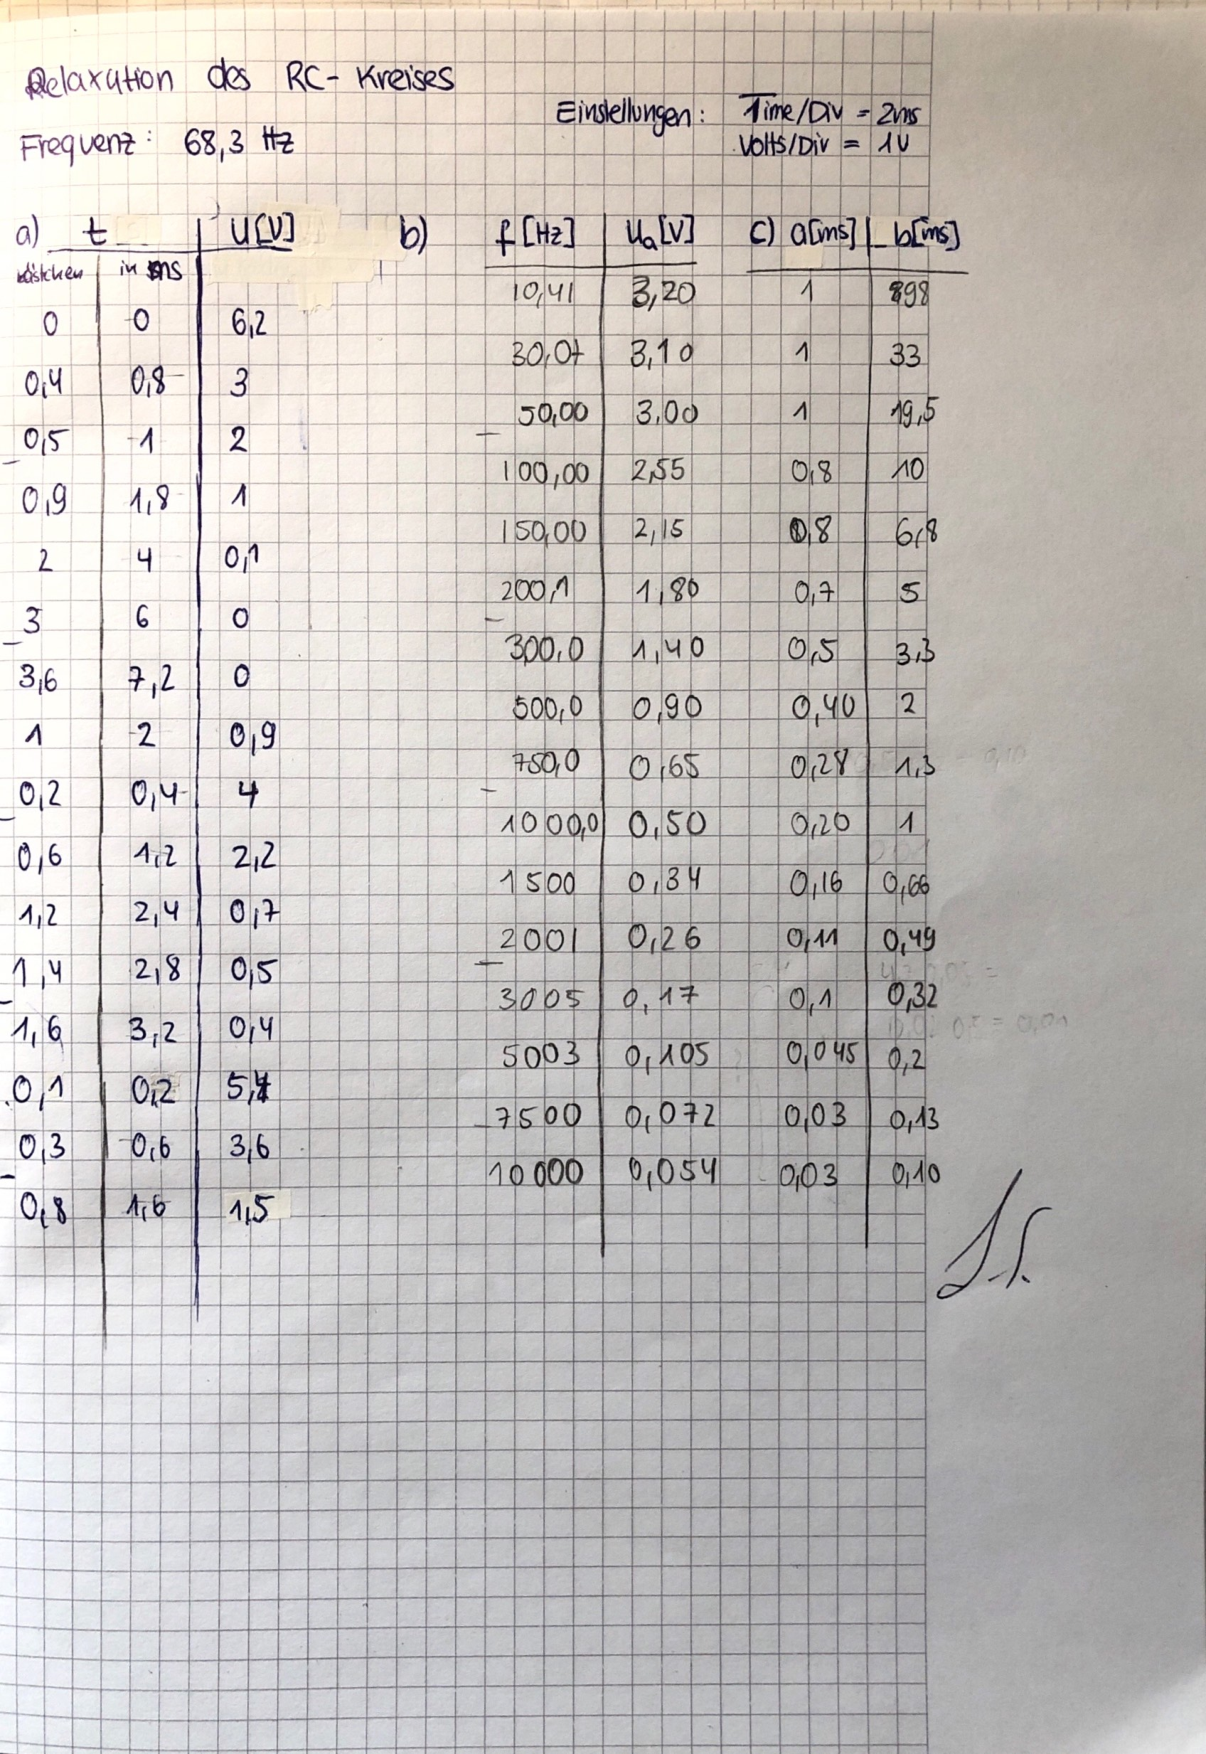
\includegraphics[width=\textwidth]{bilder/daten_V353.pdf}
    \caption{Die Originaldaten von der Versuchsdurchführung.}
\end{figure}